\section{Overview}
\subsection{Purpose}
This document contains pertinent information for the architecture and
implementation of Acme Corporation's network upgrade, including details over 
topology, services, and high-level configuration descriptions where applicable.
\subsection{Services}
All existing services must be upgraded to accommodate the network upgrade. 
The scope of each service upgrade will vary based on the need, but each
service will be reimplemented to better fit within the post-upgrade network 
architecture. 
\subsubsection{Existing Services}
The following existing services will be upgraded (in no particular order):
\newcolumntype{P}[1]{>{\centering\arraybackslash}p{#1}}
\begin{center}
\begin{tabular}{|P{7.3cm}|P{5.5cm}|}
    \hline
    \textbf{Service Description} & \textbf{Preferred Package/Application} \\
    \hline
    Network File System (NFS) & nfs-kernel-server, nfs-client \\
    \hline
    Webserver & apache2 \\
    \hline
    Database & mariadb \\
    \hline
    Email & ??? \\
    \hline
    Active Directory (AD) & openldap \\
    \hline
    Domain Name Server (DNS) & \textcolor{red}{-\$30,000} \\
    \hline
    Dynamic Host Configuration Protocol (DHCP) & dhcpd \\
    \hline
\end{tabular}
\end{center}

%%%%%%%%%%%%%%%%%%%%%%%%%%%%%%%%%%%%%%%%%%% start of database writeup %%%%%%%%%%%%%%%%%%%%%%%%%%%%%%%%%%%%%%%%%%%%%%%%%% 

\subsubsection{Database}
We are going with a MariaDB database for ACME as it widely used, easily maintainable, and secure. In order to set up the MariaDB database we would need to install it both the client and server packages.

\begin{itemize}

\item sudo apt-get install mariadb-server

\end{itemize}

\noindent After running the installation of MariaDB we then would need to set up our admin user so we are then able to populate the database with data that ACME CORP needs to be stored. 

\noindent By running:

\begin{itemize}
\item sudo mysql\_secure\_installation \\
\end{itemize}

\noindent We are able to do all of the following: 

\begin{itemize}
\item set root password
\item disable remote root login
\item remove test database
\item remove anonymous users and
\item reload privileges
\end{itemize}

\noindent After adding the data that needs to be stored we would then set up the user accounts and privileges for the HR department as they are the only department needing access to the database.

\begin{itemize}

\item MariaDB $>$ CREATE USER frankHR@'localhost' IDENTIFIED BY 'password'

\item MariaDB $>$ GRANT ALL PRIVILEGES on employees.* to frankHR@'\%';

\item MariaDB $>$ FLUSH PRIVILEGES; 

\end{itemize}

\noindent By the above commands we created a user account from Frank from HR and then have given Frank privileges to access the database 'employees'. Following this same style we would be able to add new tables and users and also give and take away privileges based on needs.

%%%%%%%%%%%%%%%%%%%%%%%%%%%%%%%%%%%%%%%%%%% end of database writeup %%%%%%%%%%%%%%%%%%%%%%%%%%%%%%%%%%%%%%%%%%%%%%%%%% 


\subsubsection{New Services}
The following new services will be implemented on the network (in no particular
order):
\newcolumntype{P}[1]{>{\centering\arraybackslash}p{#1}}
\begin{center}
\begin{tabular}{|P{7.3cm}|P{5.5cm}|}
    \hline
    \textbf{Service Description} & \textbf{Preferred Package/Application} \\
    \hline
    Virtual Local Area Network (VLAN) & vlan \\
    \hline
    Configuration Management & puppet \\
    \hline
    Monitoring & nagios \\
    \hline
    Virtual Private Network (VPN) & openvpn \\
    \hline
\end{tabular}
\end{center}
\subsection{Architecture}
\subsubsection{Architecture Overview}
\subsubsection{Network Topology}
\begin{figure}[!htb]
	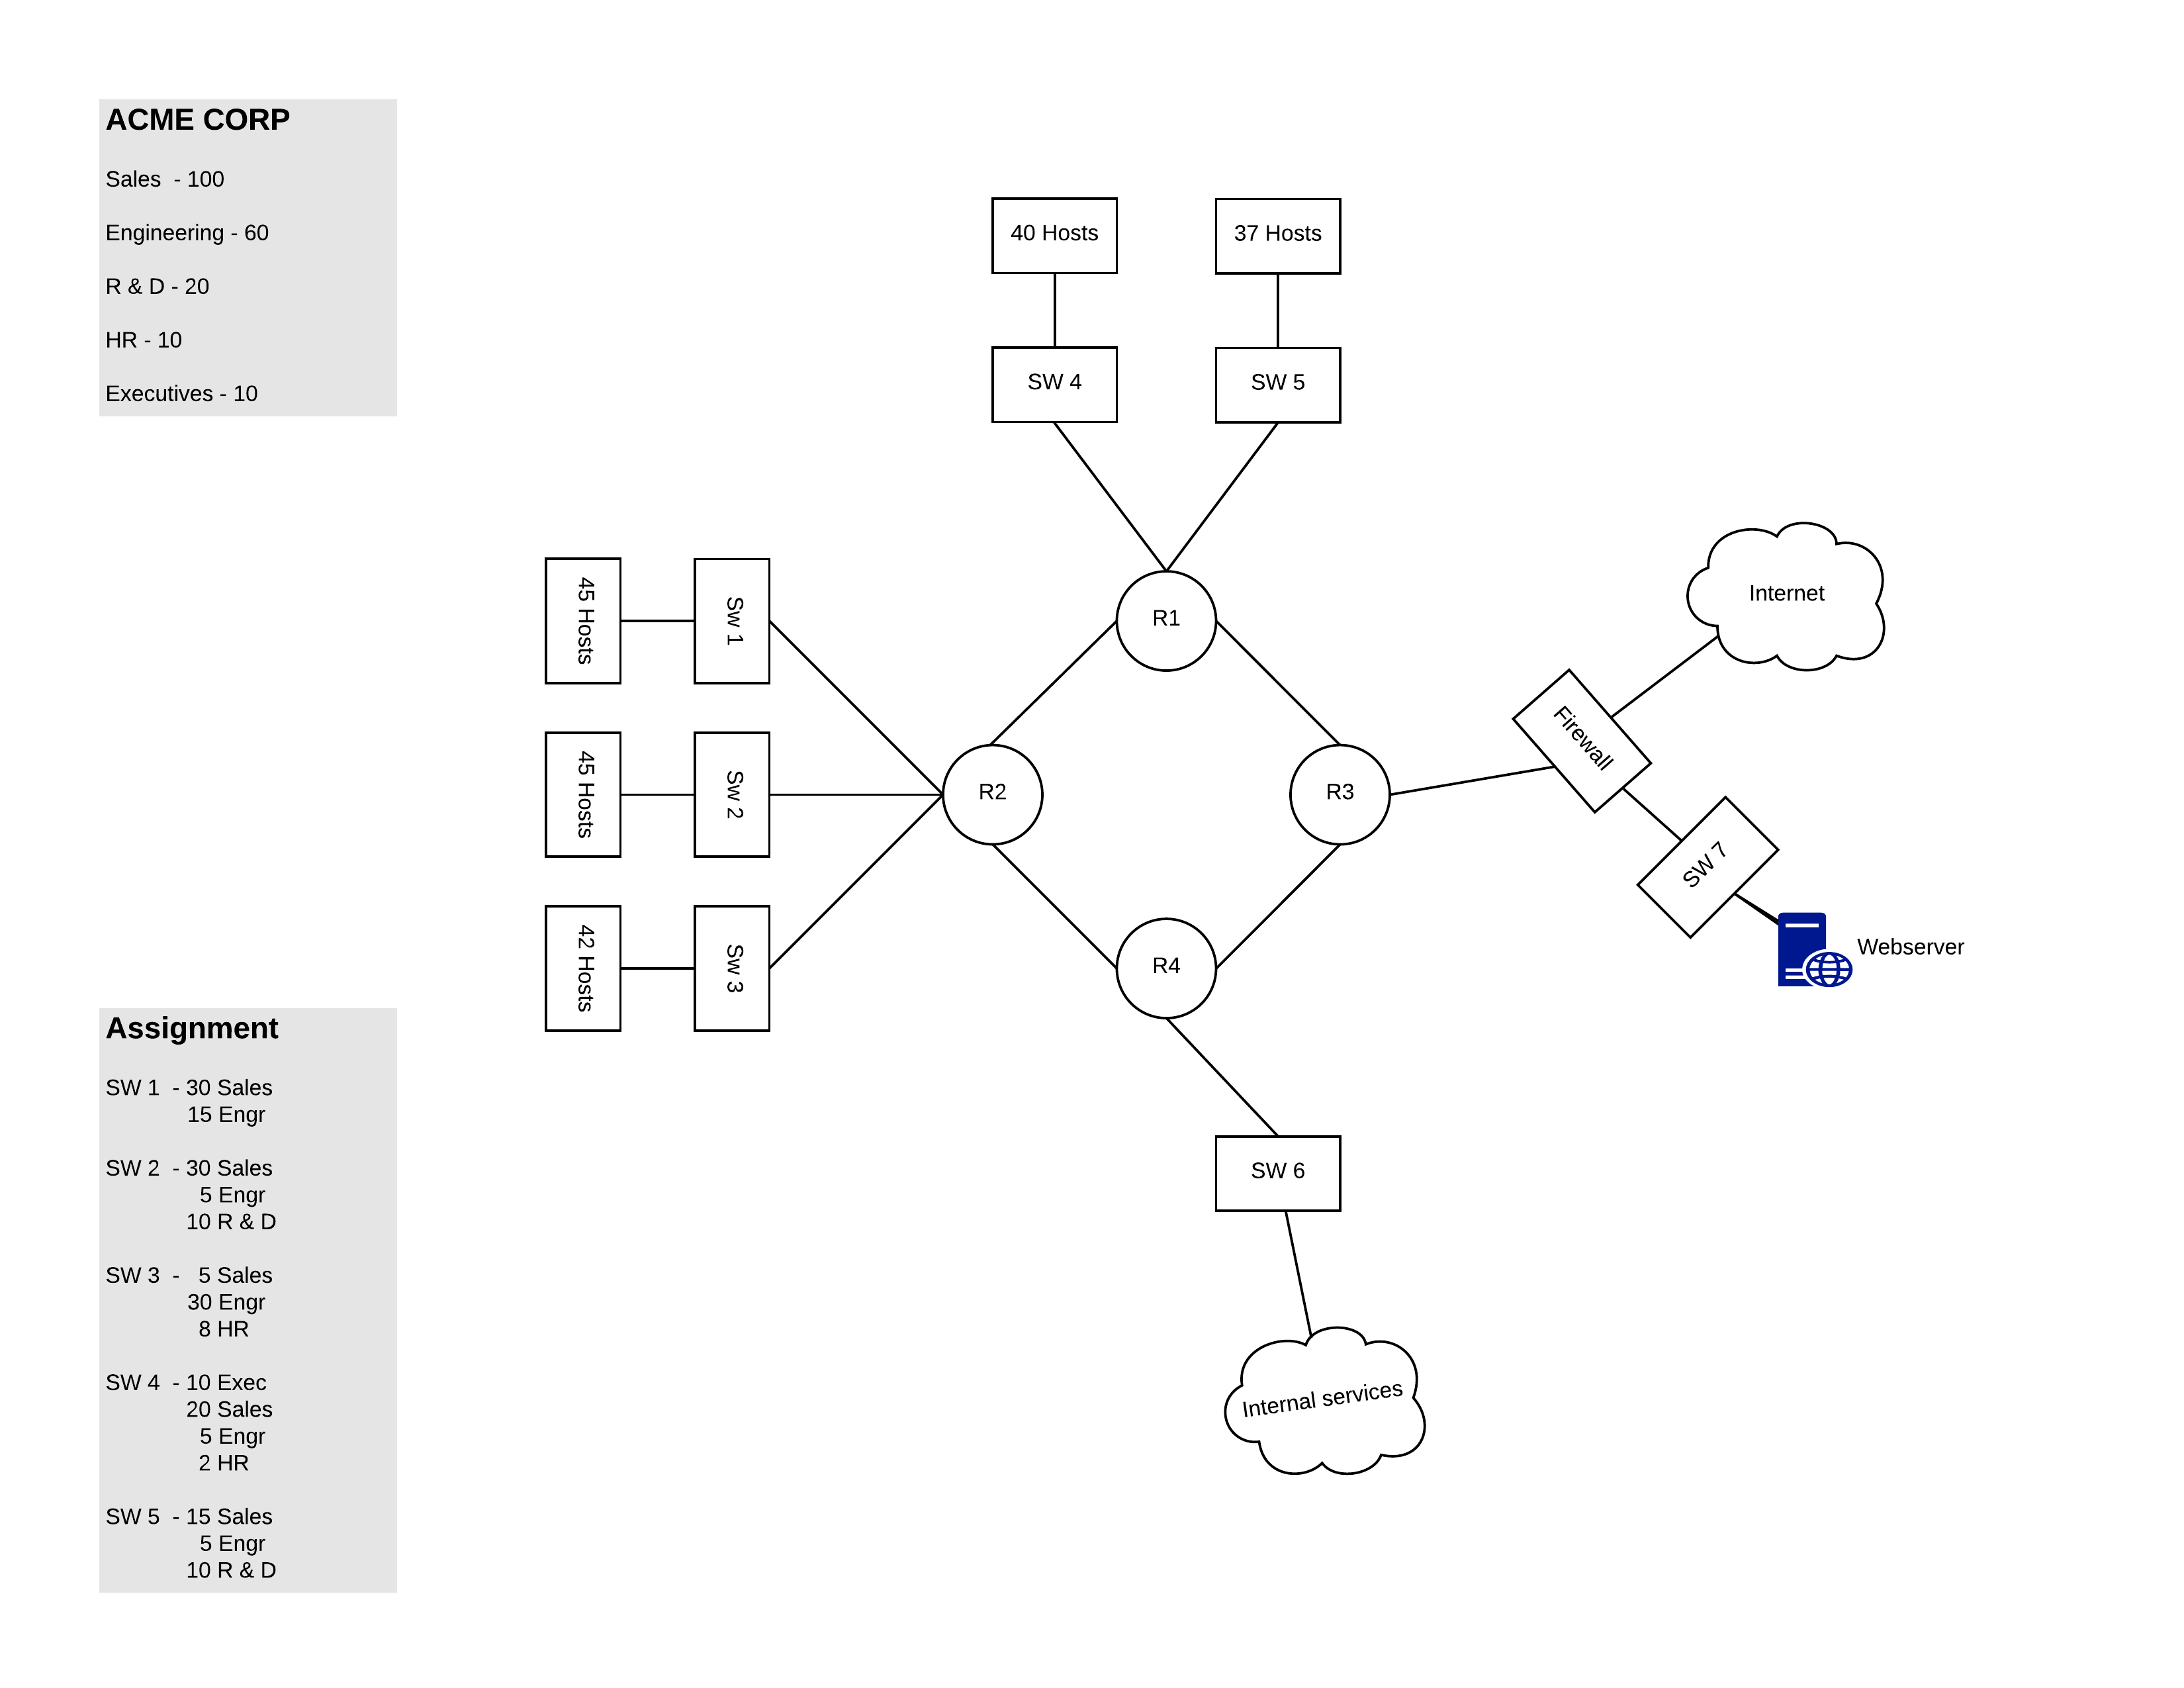
\includegraphics[width=\textwidth]{images/networktopology.png}
	\caption{Topology for ACME CORP. Network}
\end{figure}
